\thispagestyle{empty}
\raisebox{-30 mm }{
  \makebox[21cm]{
    \raggedleft                       
    \fontsize{24.88}{30} \bfseries Paper
    \colorbox{black}{
      \framebox[3cm][l]{
        \color{white}{\null\hspace{-3pt}II}
        \rule[-8pt]{0pt}{36pt}        
      }
    }
  }
}
\vspace{-7pt}

\noindent
\rule[1mm]{412pt}{2pt}
\\{}\\
\PaperII
\addcontentsline{toc}{chapter}{Paper II}
\clearpage\mbox{}\thispagestyle{empty}\clearpage
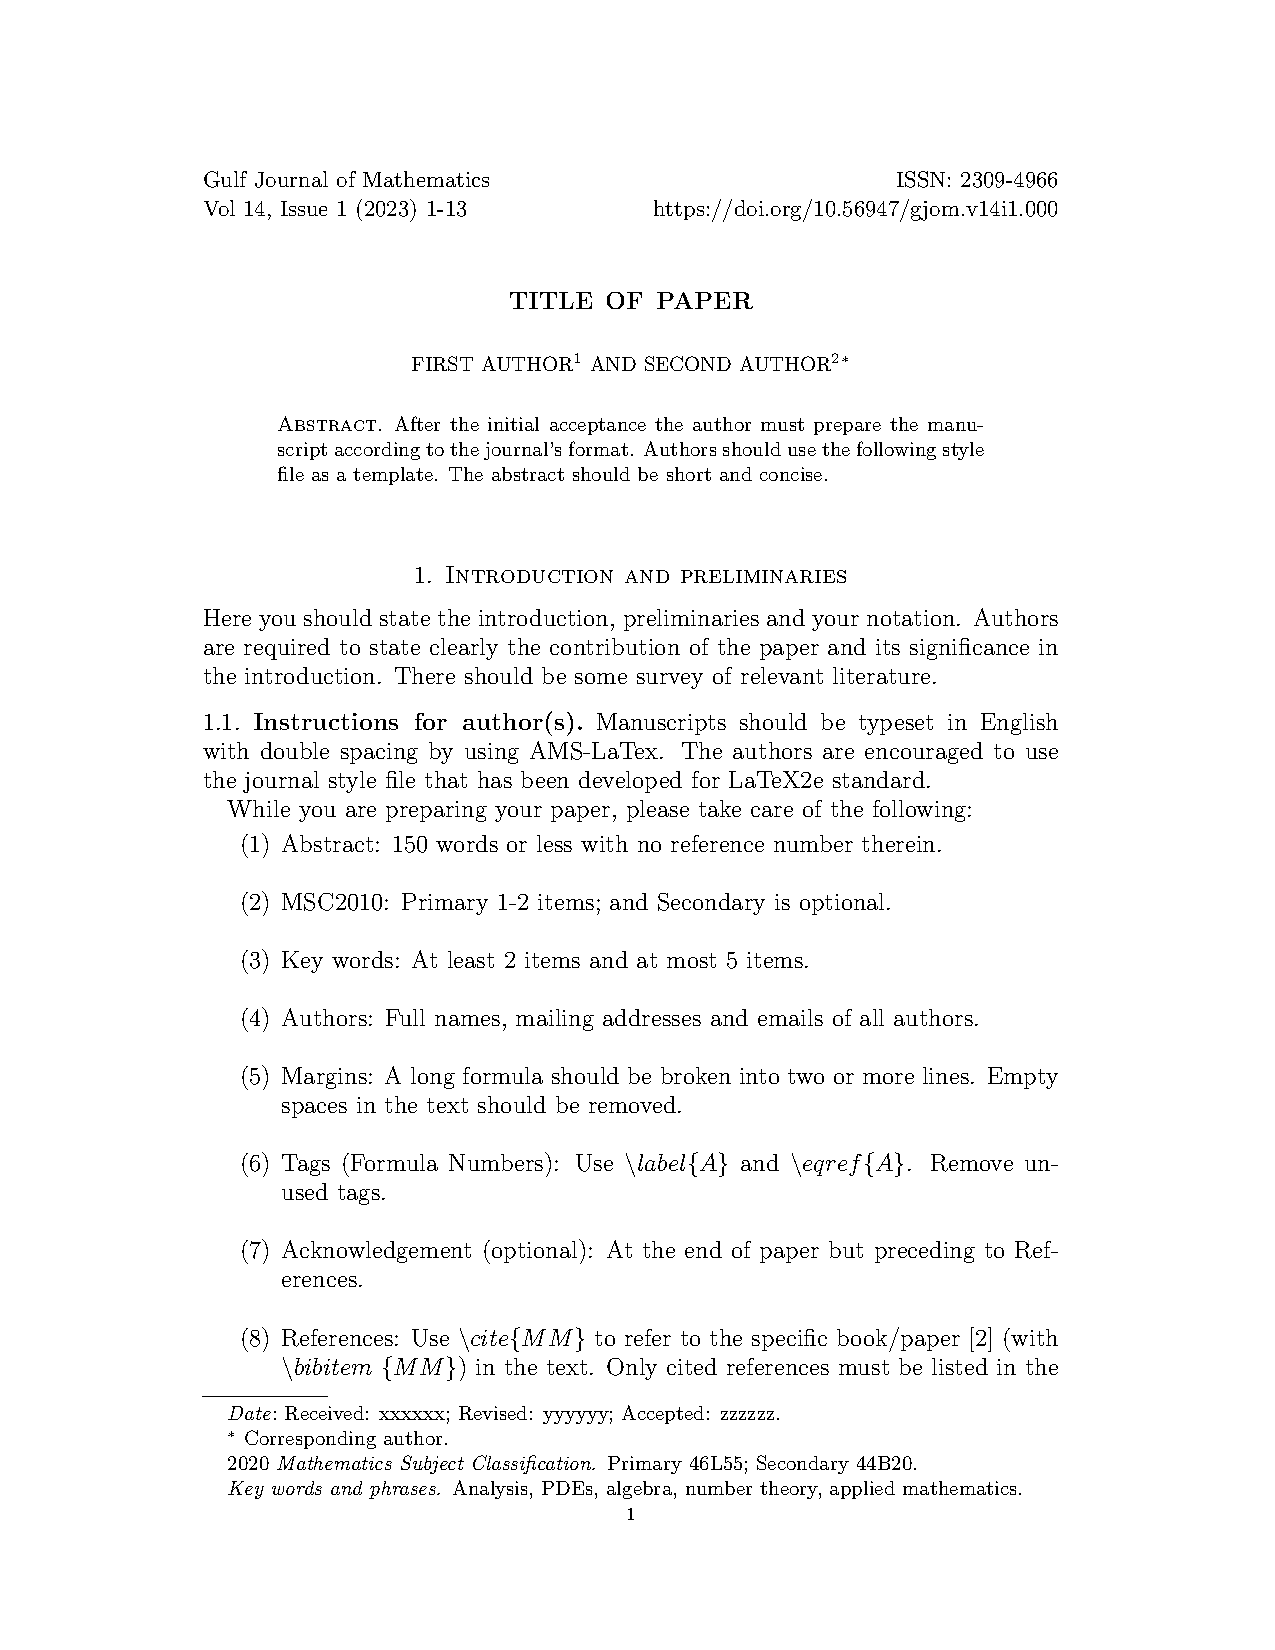
\includepdf[pagecommand={\thispagestyle{plain}}, pages={-},nup=1x1,offset = 0in 0in,frame=false, clip=true]{papers/author2024second.pdf}
% ,trim=0 105 0 100 can be used to cut out parts of the paper, as in 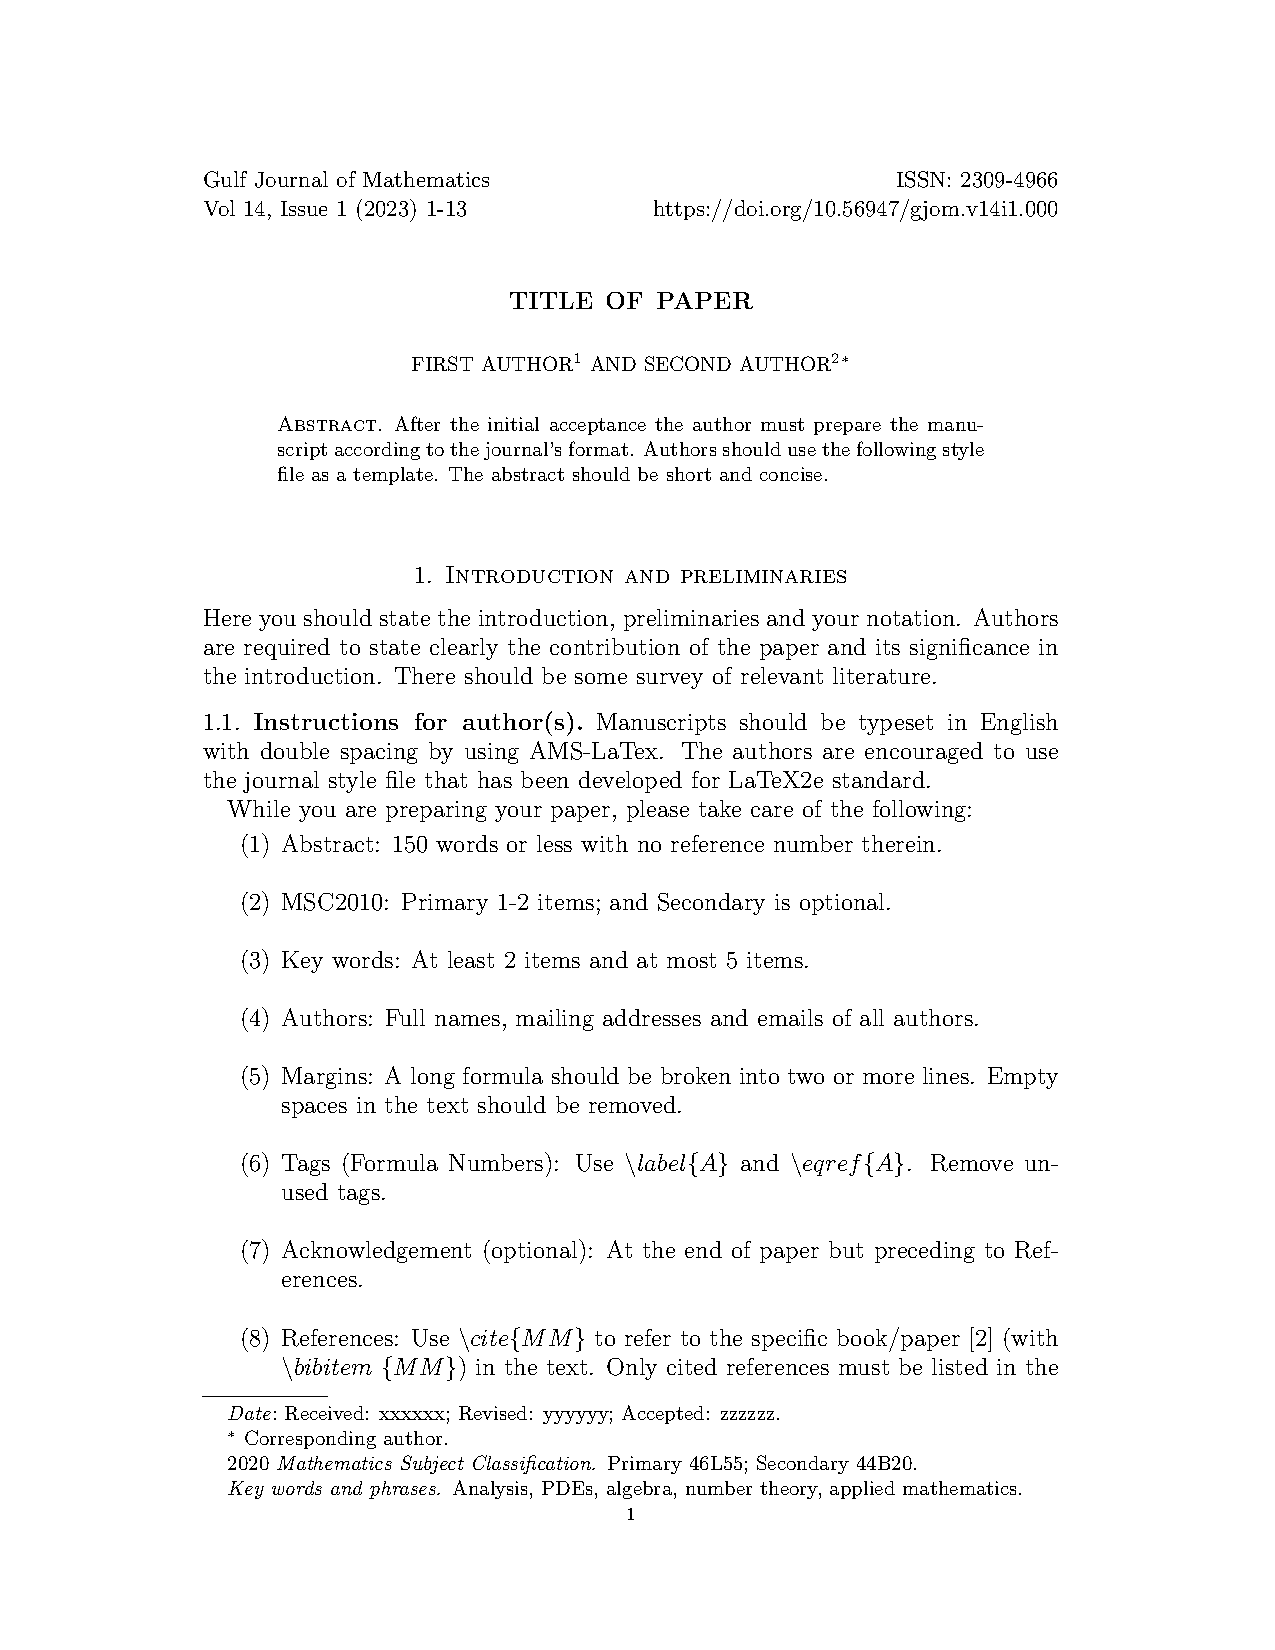
\includepdf[pagecommand={\thispagestyle{plain}}, pages={-},nup=1x1,offset = 0in 0in,frame=false,trim=0 105 0 100, clip=true]{papers/author2024second.pdf}
\clearpage